\chapter{Аналитическая часть}

В этом разделе представлен анализ предметной области, а также сравнительный обзор существующих решений. Формулируются требования к разрабатываемой базе данных и приложению, проводится формализация и описание данных, которые будут храниться в проектируемой БД. Кроме того, анализируются существующие модели баз данных, приводится диаграмма сущность-связь проектируемой системы, описываются типы пользователей и строится диаграмма прецедентов.

\section{Анализ предметной области}

Современные транспортные системы требуют эффективных инструментов для контроля и анализа перемещений автомобилей. Города активно оснащаются разветвленными сетями камер видеонаблюдения, которые в режиме реального времени фиксируют движение транспорта. Сервис, основанный на данных с уличных камер видеонаблюдения, позволяет точно отслеживать маршруты транспортных средств, обеспечивая безопасность дорожного движения и улучшение городского управления.

Технологической основой таких сервисов являются решения для автоматического распознавания номеров (Automatic License Plate Recognition, ALPR), которые позволяют идентифицировать транспортные средства по их государственным регистрационным знакам. Современные ALPR-системы достигают точности распознавания до 96.2\% даже в сложных условиях освещения и при различных углах обзора камер~\cite{ALRP}.

\section{Анализ существующих решений}

В качестве существующих решений были выбраны Flock Safety~\cite{fl-safe}, Plate Recognizer~\cite{pl-rc} и City Point~\cite{city-point}.

Для сравнения существующих решений были выбраны следующие критерии:

\begin{itemize}[label=---]
    \item КР1 --- история перемещений;
    \item КР2 --- интеграция с городскими камерами;
    \item КР3 --- гибкие фильтры поиска;
    \item КР4 --- визуализация маршрутов на карте;
    \item КР5 --- мобильное приложение;
    \item КР6 --- возможность отслеживания личного автомобиля для пользователей.
\end{itemize}

Сравнение существующих решений представлено в таблице~\ref{tbl:entity}.

\begin{table}[H]
    \begin{center}
        \caption{Сравнение существующих решений}
        \begin{tabular}{|c|c|c|c|c|c|c|}
            \hline
            \textbf{Решение} & \textbf{КР1} & \textbf{КР2} & \textbf{КР3} & \textbf{КР4} & \textbf{КР5} & \textbf{КР6}\\
            \hline
            Flock Safety & + & + & + & + & - & - \\
            \hline
            Plate Recognizer & + & + & + & - & - & - \\
            \hline
            City Point & + & + & + & + & - & + \\
            \hline
        \end{tabular}
        \label{tbl:entity}
    \end{center}
\end{table}

По результатам сравнения, ни одно из рассмотренных решений не удовлетворяет всем выдвинутым критериям.

\section{Анализ моделей баз данных}

База данных (БД) --- совокупность данных, организованных по определенным правилам, предусматривающим общие принципы описания, хранения иманипулирования данными, независимая от прикладных программ~\cite{bd-def}.

Модель данных — это абстрактное, самодостаточное, логическое определение объектов, операторов и прочих элементов, в совокупности составляющих абстрактную машину доступа к данным, с которой взаимодействует пользователь. Упомянутые объекты позволяют моделировать структуру данных, а операторы — поведение данных~\cite{model-def}.

По модели данных базы данных разделяют на следующие категории:
дореляционные, реляционные и постреляционные.

\subsection{Дореляционные базы данных}

Являются предшественниками реляционных баз данных. Такие системы не основывались на каких-либо абстрактных моделях, а также такие системы не основывались на каких-либо абстрактных моделях~\cite{models}.

Основным преимуществом данных моделей является возможность построения вручную эффективных прикладных систем.

Недостатками данных моделей являются необходимость знания о физической организации, а также перегруженность деталями организации доступа.

\subsection{Реляционные базы данных}

Реляционная база данных – это набор данных с заданными взаимосвязями.

Реляционная модель объединяет данные в таблицы, где каждая строка представляет собой отдельную запись, а каждый столбец состоит из атрибутов, содержащих значения~\cite{model-def}.

Основными преимуществами данной модели являются:

\begin{itemize}[label = ---]
    \item поддержка языка запросов SQL;
    \item отображение информации в наиболее простой для пользователя форме;
    \item представление сущностей единым образом в виде отношений.
\end{itemize}

Основным недостатком данной модели является медленный доступ к данным среди всех моделей данных;

\subsection{Постреляционные базы данных}

Классическая реляционная модель предполагает неделимость данных, хранящихся в полях записей таблиц. Существует ряд случаев, когда это ограничение мешает эффективной реализации приложений.

Постреляционная модель данных представляет собой расширенную реляционную модель, снимающую ограничение неделимости данных, хранящихся в записях таблиц. Постреляционная модель допускает многозначные поля --- поля значение которых состоит из подзначений. Помимо обеспечения вложенности полей постреляционная модель поддерживает ассоциированные многозначные поля.

Основным достоинством постреляционной модели является возможность представления совокупности связанных реляционных таблиц в виде одной постреляционной таблицы.

Недостатками данной модели являются отсутствие стандартизированных языков запросов и общепринятой модели, а также сложность обеспечения
целостности.

\section{Выбор модели базы данных}

Так как данные обладают строгой структурой, не подвержены частым изменениям, а также предполагается выполнение запросов различной сложности и необходимость обеспечения независимости хранения информации от приложения, было принято решение использовать реляционную модель базы данных.

\section{Формализация ролей}

Исходя из поставленной задачи и особенностей предметной области, следует выделить три основных типа пользователей:

\begin{itemize}[label=---]
    \item \textbf{пользователь} должен обладать следующими возможностями:
    \begin{itemize}[label=---]
        \item регистрация;
        \item авторизация;
        \item просмотр маршрутов автомобилей;
    \end{itemize}
    \item \textbf{оператор} должен обладать следующими возможностями:
    \begin{itemize}[label=---]
        \item авторизация;
        \item поиск маршрутов об отслеживании по критериям;
        \item просмотр маршрутов автомобилей;
    \end{itemize}
    \item \textbf{аудит} должен обладать следующими возможностями:
    \begin{itemize}[label=---]
        \item авторизация;
        \item поиск информации об отслеживании по критериям;
        \item просмотр информации об отслеживании.
    \end{itemize}
\end{itemize}

На рисунке~\ref{fig:use-case} представлена диаграмма прецедентов.

\begin{figure}[H]
    \centering
    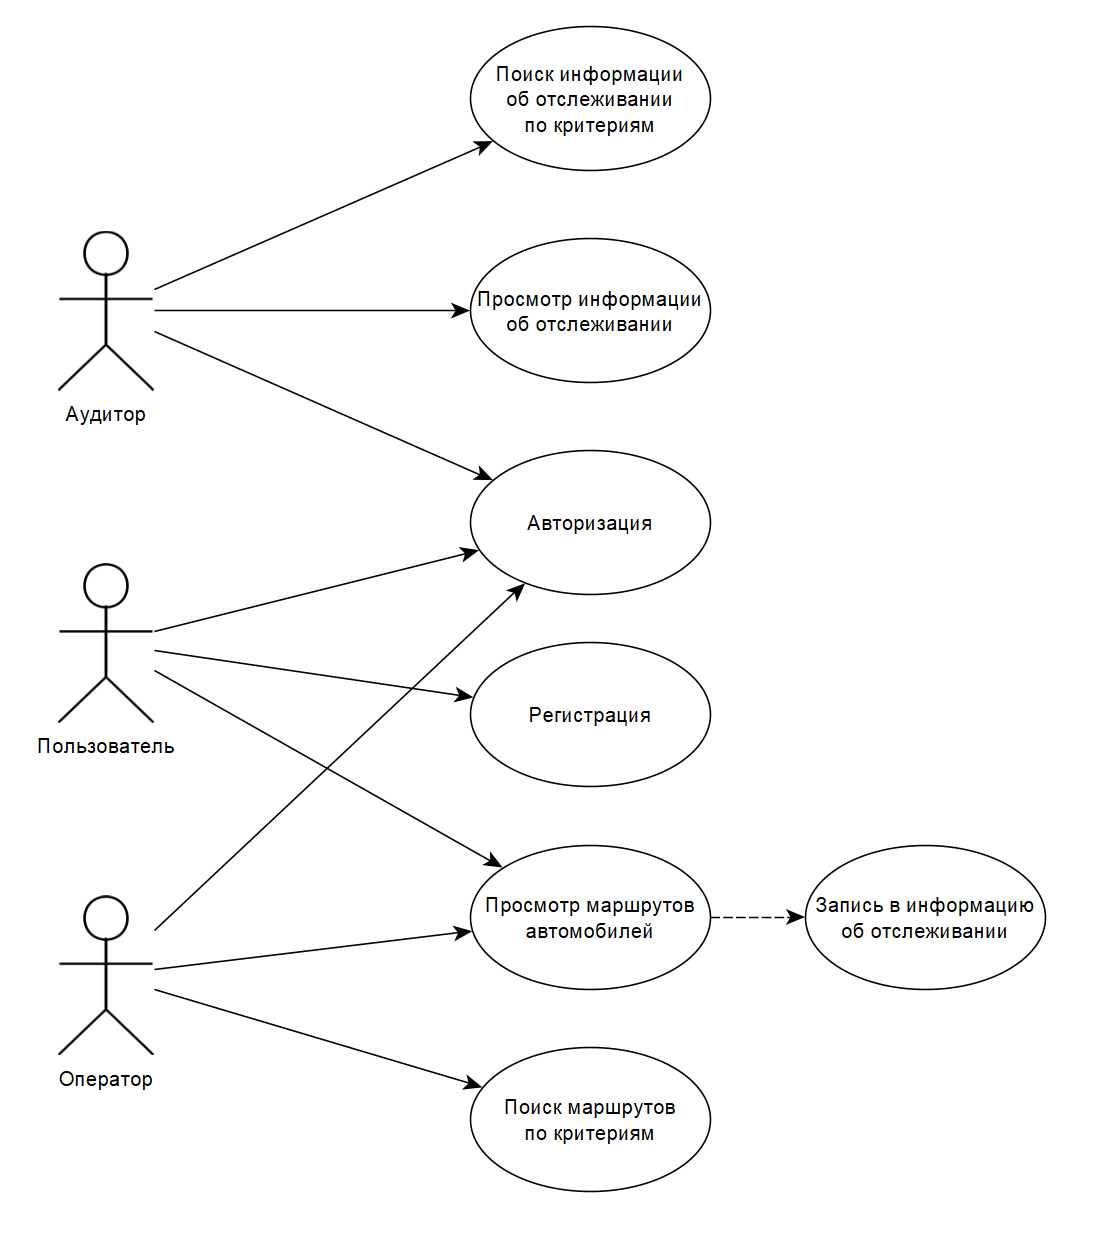
\includegraphics[width=0.8\linewidth]{images/diograms/use_case.png}
    \caption{Диаграмма прецедентов}
    \label{fig:use-case}
\end{figure}

\section{Формализация данных}

База данных должна содержать информацию о:

\begin{itemize}[label=---]
    \item пользователь;
    \item информация об отслеживании;
    \item транспортное средство (ТС);
    \item свидетельство о регистрации ТС (СТС); 
    \item паспорт ТС (ПТС);
    \item владелец;
    \item история владельцев;
    \item камера;
    \item снимок.
\end{itemize}

Сведения о каждой сущности содержится в таблице~\ref{table:entity}.

\begin{table}[H]
    \begin{center}
        \caption{Сведения о категориях данных}
        \begin{tabular}{|c|c|}
            \hline
            \textbf{Сущность} & \textbf{Информация} \\
            \hline
            Пользователь & \makecell{ФИО, паспорт, \\ логин, пароль, роль} \\
            \hline
            \makecell{Информация \\ об отслеживании} & \makecell{Время, дата, \\дата маршрута} \\
            \hline
            ТС & \makecell{Цвет, VIN, марка, модель, \\ тип кузова, пробег} \\
            \hline
            СТС & \makecell{Масса, тип двигателя, номер \\ лошадиные силы, модель, марка, \\ дата постановки, год выпуска, ГРЗ, \\ VIN, категория ТС} \\
            \hline
            ПТС & \makecell{страна ввоза, номер} \\
            \hline
            Владелец & \makecell{Возраст, ФИО, ВУ, \\паспорт, стаж вождения} \\
            \hline
            История владельцев & \makecell{Дата постановки на учет, \\ дата снятия с учета, пробег} \\
            \hline
            Камера & \makecell{Наличие радара, дата установки,\\ширина, долгота} \\
            \hline
            Снимок & \makecell{Полоса, время, дата, \\ скрость, ГРЗ} \\
            \hline
        \end{tabular}
        \label{table:entity}
    \end{center}
\end{table}

На рисунке~\ref{fig:er_diogramm} приведена диаграмма сущность-связь в нотации Чена.

\begin{figure}[H]
    \centering
    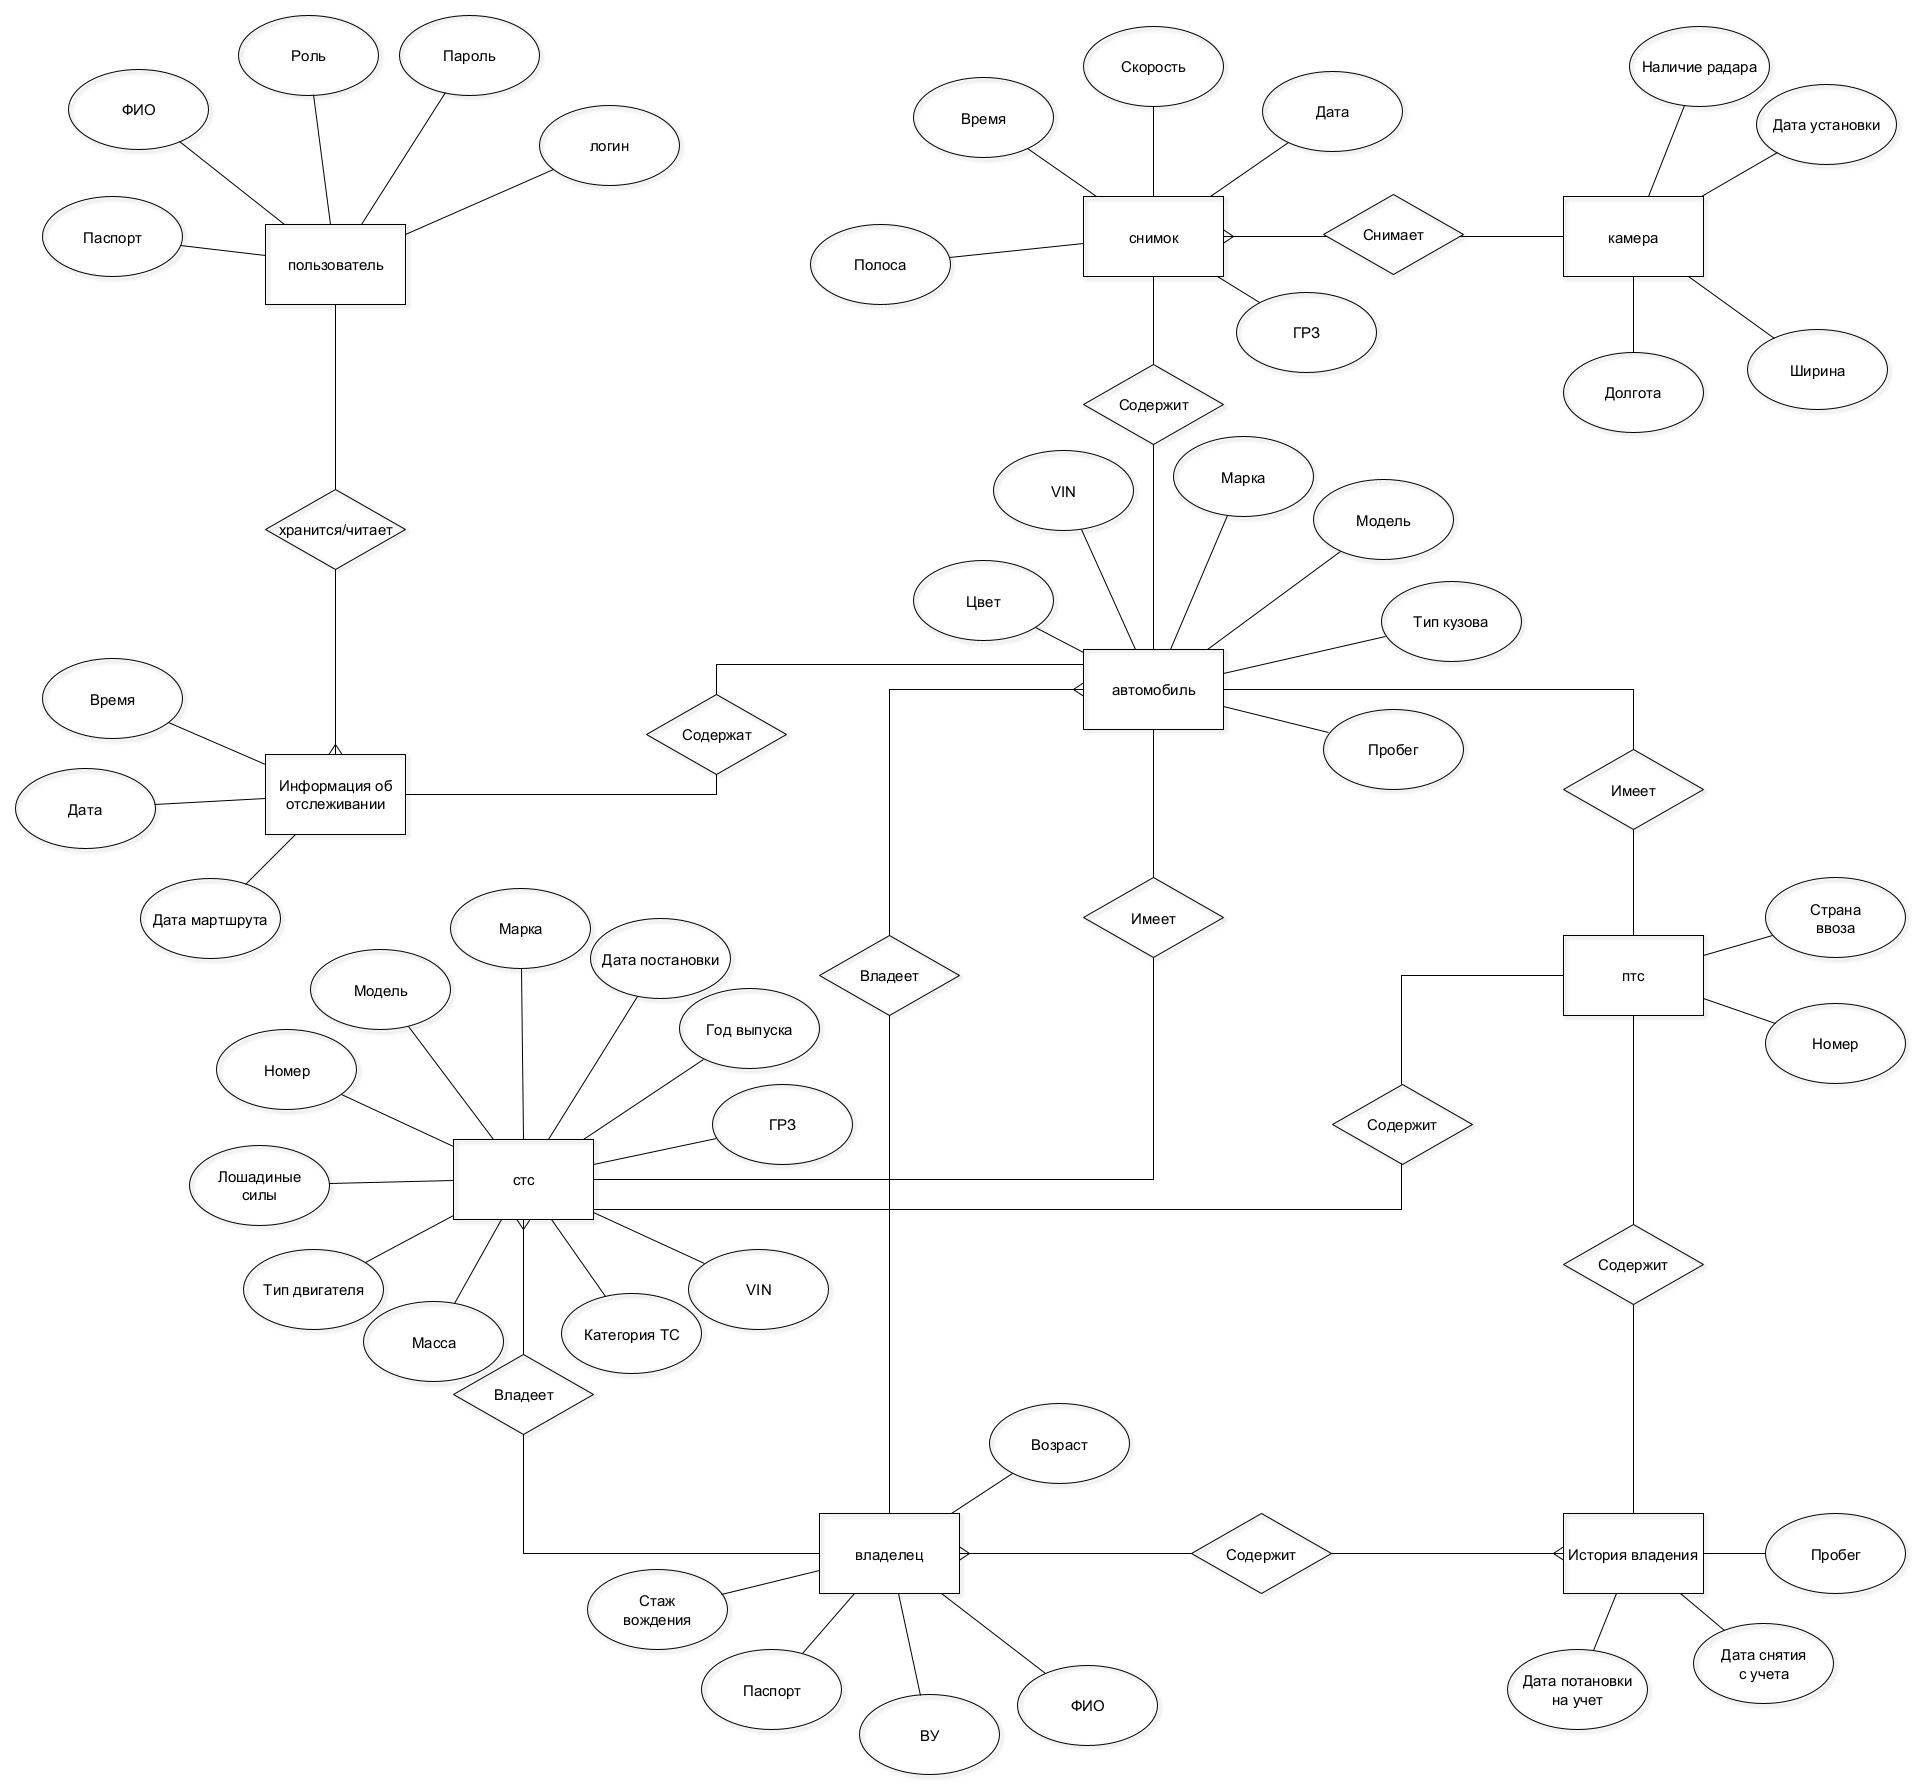
\includegraphics[width=1\linewidth]{images/diograms/er.jpg}
    \caption{Диаграмма сущность-связь}
    \label{fig:er_diogramm}
\end{figure}

\section{Формализация задачи}

Требуется спроектировать базу данных для хранения сведений о пользователях, автомобилях, владельцах, снимках и камерах. Также необходимо разработать приложение с интерфейсом для просмотра данных, содержащихся в базе. Предусматривается реализация трех ролей с различными уровнями доступа: пользователь, оператор и аудитор.

\paragraph*{ВЫВОД} ${}$ \\

В данном разделе представлен анализ предметной области и проведено сравнение существующих решений. Сформулированы требования к разрабатываемой базе данных и приложению, а также выполнена формализация и описание информации, подлежащей хранению в базе данных. Кроме того, рассмотрены существующие модели баз данных и представлена диаграмма сущность-связь для проектируемой системы. Также описаны типы пользователей и приведена диаграмма прецедентов.
